In this section the compact models presented in chapter \ref{chapter:compact-models} focusing in particular of MTZ and its variants and GG models. To test them a set of 20 instance of 50 nodes were generated and runned with a global timelimit of 30 minutes. The results are visible in figure \ref{fig:result-compact}.

\begin{figure}[h]
	\centering
	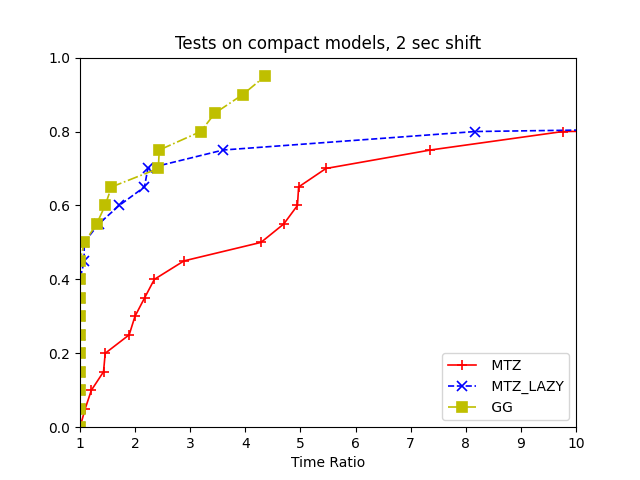
\includegraphics[width=0.6\textwidth]{images/final_mtz_mtzlazy_gg.png}
	\caption{The comparison chart of the compact models.}
	\label{fig:result-compact}
\end{figure}

From this image we can state that the MTZ basic model is far from being the best one of this section. In fact the best models are GG and MTZ\_LAZY wich on many instaces perform in a comparable way. But it is possible to see that while MTZ\_LAZY in some cases as reached the timelimit, the GG model deliver a consistent solution of the instance.